\chapter{UCN Production and Detection}

The first UCN at TRIUMF (Nov.~2017) were produced by using the
vertical UCN source described in Sec.~\ref{vertical_source}. The
spallation neutrons were converted to UCN through phonon excitation in
the isotopically pure superfluid helium.  During data taking several
measurements were performed for better understandting of the vertical
UCN source to design the next generation UCN source. In this chapter,
the experiments are described and the result are shown.

The Tungsten target is irradiated by the proton beam for a certain
amount of time. To accumulate UCN, the gate valve shown in Fig.~ (???)
must be closed during this time. A typical UCN cycle of measuremet
starts at the end of the irradiation time. After the irradiation
stops, the gate valve is opened and the UCN can reach the detector to
measure the UCN yield. When the valve is opened, the UCN rate goes up
and it eventually decays down to the background rat~(less than 3
UCN/s) as shown in Fig.~\ref{fig:UCNRate}.

\begin{figure}[h]
  \centering
  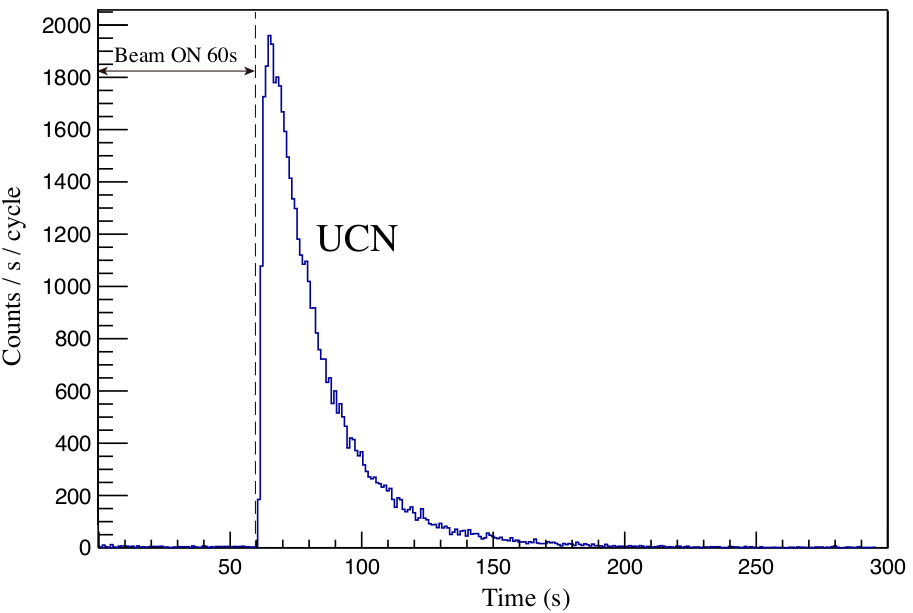
\includegraphics[width=0.7\textwidth]{UCNRate.png}
  \caption{The figure shows the UCN rate at 60~s irradiation time and
    1~$\mu$A beam current. In this case, the UCN gate valve is opened
    immediately after the end of irradiation. At this time, the UCN
    rate reaches the peak of about 2000 UCN/s. The UCN rate decays
    down to zero. The Valve is left open for 120~s. }
  \label{fig:UCNRate}
\end{figure}



The total number of UCN can be analytically calculated using
differential equations.  Consider a volume $V_1$ to be the production
volume~(In the case of TUCAN experiment shown in
Fig.~\ref{fig:Source_all}, it is the superfluid helium volume and and
the horizontal guide section before the gate valve.) with $N_1$ number
of UCN, and $V_2$ to be the secondary volume where $N_2$ UCN enters
after opening the valve~(from the UCN gate valve to the main detector
as shown in Fig.~\ref{fig:Source_all}), and $V_3$ be the detector
volume with $N_3$ numberof neutrons~(See
Fig.~\ref{fig:volume_schematic}).



\begin{figure}[h]
  \centering
  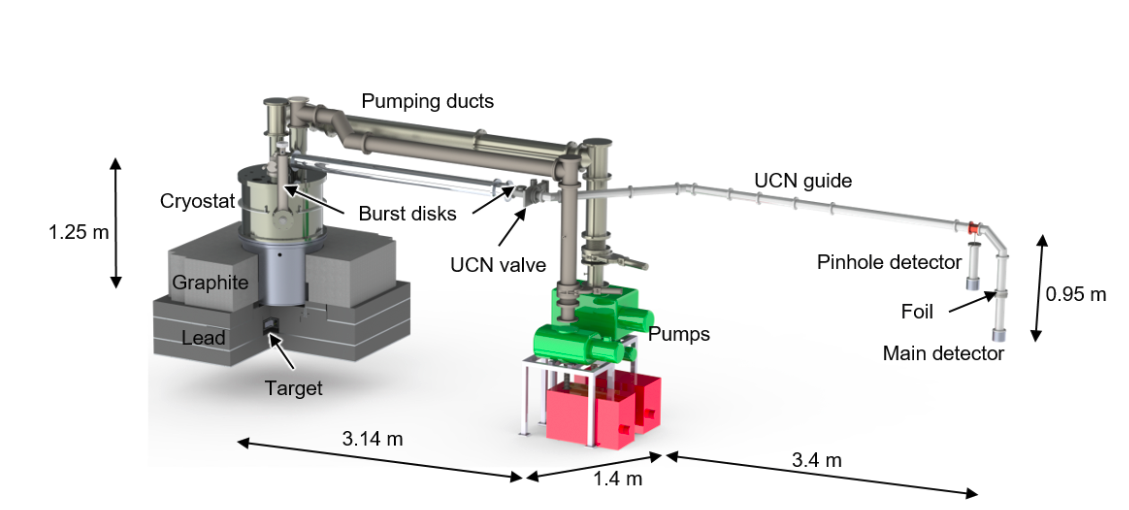
\includegraphics[width=1.1\textwidth]{Source_all.png}
  \caption{The UCN source and the guide geometry at TRIUMF }
  \label{fig:Source_all}
\end{figure}






\begin{figure}[h]
  \centering
  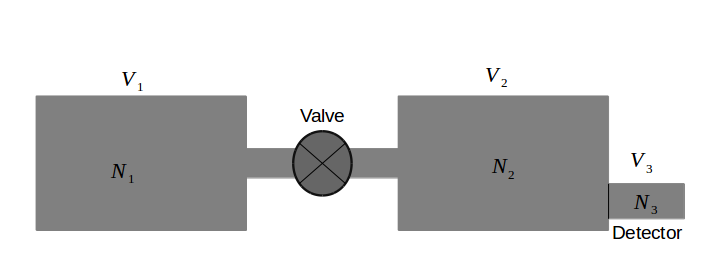
\includegraphics[width=0.9\textwidth]{volume_schematic.png}
  \caption{Schematic drawing of a UCN source. $V_1$ is the production
    volume with $N_1$ number of UCN, $V_2$ is the secondary volume
    where $N_2$ number of UCN exist and $V_3$ is the detector with
    $N_3$ number of UCN. }
  \label{fig:volume_schematic}
\end{figure}



When the UCN gate valve is closed and the beam is on, the changes in
the UCN counts $N_1$ over time can be described by the equation below:

\begin{equation}
\frac{dN_1}{dt} = P - \frac{N_1}{\tau_1}  
\end{equation}

Where $P$ is the UCN production rate as describe in
Sec.~\ref{sec:UCN_production} and $\tau_1$ is the UCN storage lifetime
in the source. After the beam is turned off and the valve is opened,
the UCN travels to the volume $V_2$. Since this is a closed volume,
the number of UCN in $V_1$ decreases while the UCN counts in $V_2$
increases. This could be described as

\begin{equation}
  \begin{aligned}
    \frac{dN_1}{dt} =&- \frac{N_1}{\tau_{c,1}} - \frac{N_1}{\tau_1} + \frac{N_2}{\tau_{c,2}}  \\
    \frac{dN_2}{dt} =& \frac{N_1}{\tau_{c,1}} - \frac{N_2}{\tau_{c,2}} - \frac{N_2}{\tau_2} - \frac{N_2}{\tau_{c,3}} \\
    \frac{dN_3}{dt} =& \frac{N_2}{\tau_{c,3}}.
  \end{aligned}
\end{equation}

In this equation, $\frac{dN_1}{dt}$ shows the change in the UCN counts
over time in $V_1$, $\frac{dN_2}{dt}$ shows the change in the UCN
counts in $V_2$ and $\frac{dN_3}{dt}$ is change in the UCN count in
$V_3$ which is the detector. After the valve is opened, some UCN get
into $V_2$~($\frac{N_1}{\tau_{c,1}}$) with the crossing rate of
$\tau_{c,1}$, and some UCN is lost with the loss rate of $\tau_1$. In
addition, some UCN can bounce back from $V_2$ to
$V_1$~($\frac{N_2}{\tau_{c,2}}$).

In $V_2$, some UCN cross from $V_1$ to
$V_2$~($\frac{N_1}{\tau_{c,1}}$), some get lost with the loss rate of
$\tau_2$~($\frac{N_2}{\tau_2}$), some cross the gate valve to go back
to $V_1$~($\frac{N_2}{\tau_{c,2}}$) and some get to the detector with
the lifetime of $\tau_{c,3}$~($\frac{N_2}{\tau_{c,3}}$). The rate of
the UCN detection $\frac{dN_3}{dt}$ is the number of UCN crossing from
$V_2$ with the crossing rate of $\tau_{c,3}$.






The total number of produced UCN $N$ at a certain time t$_i$ can be
described by
\begin{equation}
  \label{eq:totalUCN}
  N = P \tau_1\left[ 1- \exp \left(\frac{t_i }{ \tau_1}\right) \right]
\end{equation}

where $P$ is the UCN production rate and $\tau_1$ is the UCN loss rate
in the source given by

\begin{equation}
  \frac{1}{\tau_1} = \frac{ f_\mathrm{He,1}}{\tau_\mathrm{He}} + \frac{1}{\tau_\mathrm{wall,1}}.
\end{equation}

Here (describe the parameters)...

First a set of UCN counts measurements is discussed. The UCN yield is
measured at different irradiation times, different beam currents and
different isotopic superfluid helium temperature. This is essential
for UCN yield optimization.  Next the UCN storage lifetime in the
source is studied at different beam currents, different irradiation
times and different temperatures of isotopically pure superfluid
helium. Over the course of the experimental run, the UCN storage
lifetime was measured on a daily basis. The idea behind this was to
look for long term changes in the source due to factors such as the
contamination in the source and to understand how long it is feasable
to run the source.






Put the rate equations here.
\section{UCN Counts Measurement}



\section{Storage Lifetime Measurements}

\section{Heater Tests of The Source}

\section{Detector Comparison}
Using the rotary valve

\section{Background Measurements}
With Ni foil

\section{UCN guide Transmission Measurements}

\section{Result And Conclusion}

%\begin{description}
%\item{I think this belongs to this chapter: UCN production by
%  multiphonon excitation in superfluid helium (I can use my candidacy
%  report for this part as a start)}
  
%\item{Some information about the detector}
  
%\item{UCN data goes here}
  
%\item{what else?}
%\end{description}
